%\documentclass{article}
%\usepackage{tikz}
%\usetikzlibrary{arrows.meta}
%\begin{document}

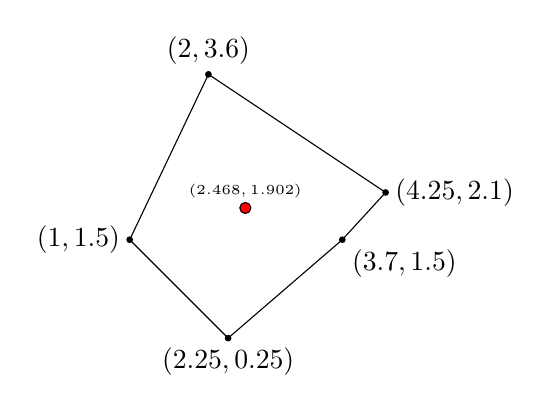
\begin{tikzpicture}
\coordinate (A) at (1,1.5);
\coordinate (B) at (2,3.6);
\coordinate (C) at (4.25,2.1);
\coordinate (D) at (3.7,1.5);
\coordinate (E) at (2.25,0.25);

\draw (A) -- (B) -- (C) -- (D) -- (E) -- (A);
\draw[fill=black] (A) circle (1pt);
\draw[fill=black] (B) circle (1pt);
\draw[fill=black] (C) circle (1pt);
\draw[fill=black] (D) circle (1pt);
\draw[fill=black] (E) circle (1pt);

\node[left]  at (A) {$(1,1.5)$};
\node[above] at (B) {$(2,3.6)$};
\node[right] at (C) {$(4.25,2.1)$};
\node[below right] at (D) {$(3.7,1.5)$};
\node[below] at (E) {$(2.25,0.25)$};

\draw[fill=red] (2.468405, 1.902874) circle (2pt);
\node[above] at (2.468405, 1.902874) {\tiny $(2.468, 1.902)$};

\end{tikzpicture}


%\end{document}

